\documentclass{class}

% Publication Title
\title{Cake classification}
% Short title for the header (copy the main title if it is not too long)
\shorttitle{Cake classification}

% Authors
\author[1]{D. Ligari 518592}
% Author Affiliations
\affil[1]{Machine Learning course, University of Pavia, Department of Computer Engineering (Data Science), Pavia, Italy}
% Surname of the first author of the manuscript
\firstauthor{Ligari}
%Contact Author Information
\contactauthor{D. Ligari} % Name and surname of the contact author
\email{davide.ligari01@universitadipavia.it} % Contact Author Email
% Publication data (will be defined in the edition)
\publicationdate{\today}
% Place your particular definitions here
\newcommand{\vect}[1]{\mathbf{#1}}  % vectors
\github{https://github.com/DavideLigari01/cake-classification}


\abstract{
 This project focuses on image recognition using two approaches: one using hand-crafted image features processed by a classification model, 
 and the other utilizing a convolutional neural network (CNN) that directly processes image pixels. 
 The lab activity involves building classifiers for cake image classification using low-level features and neural features extracted from
 the 'PVMLNet' CNN.
 Transfer learning is explored by replacing the last layer of PVMLNet with a trained perceptron. 
 The assignment involves refining the lab activity scripts and performing additional exercises, 
 such as combining different features, analyzing class confusion, and exploring different hidden layers for neural features.
 Overall, the project explores various techniques and models for image recognition and aims to improve classification accuracy.}
\keywords{ MLP Neural network • Convolutional neural network • Low level features • Confusion matrix}
\date{\today}
% Start document
\begin{document}
\maketitle
\thispagestyle{FirstPage}
\pagenumbering{arabic}
\section{Introduction}
\firstword{C}{onvolutional}
neural networks (CNNs) have revolutionized image recognition, enabling computers to understand and classify visual data with remarkable accuracy.
Unlike traditional methods that rely on manual feature engineering, CNNs can automatically learn and extract meaningful features directly from raw image pixels.
This ability to capture spatial relationships and hierarchies of features has made CNNs the go-to approach for tasks such as object detection and image classification.
In this project, the effectiveness of CNNs is explored for the classification of cake images, comparing them with hand-crafted feature approaches.
The goal is to leverage the power of deep learning and investigate the potential of transfer learning in improving classification accuracy.

\section{Lab activity}
\subsection{Low-level features -- Write a script that computes one of the low-level feature vector implemented in the
    image features.py file. Train a classifier and evaluate the test accuracy.}
The chosen low-level feature vector for the classification task is the histogram of the color image.
To train the model, an MLP neural network without hidden layers was utilized, with parameters set as follows: 5000 epochs, a batch size of 50,
and a learning rate of 0.0001.\\
Figure \ref{fig-1} illustrates the train and test accuracy trends over the epochs.
However, the results reveal the model's poor predictive capabilities, as both the train and test accuracy remain below 22\%.
It can be inferred that the model is underfitting the data. To enhance its predictive ability,
it is recommended to introduce intermediate levels or hidden layers to increase the complexity of the model.
This will allow the network to capture more intricate patterns and improve its classification performance.
\begin{figure}[h]
    \centering
    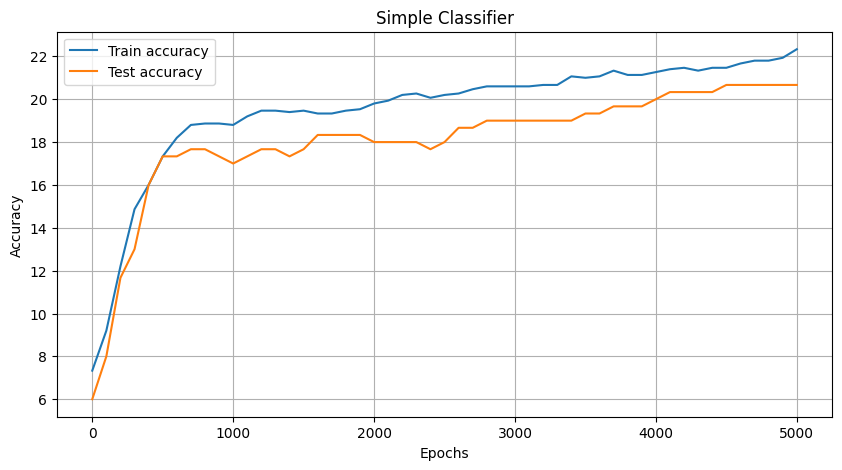
\includegraphics[width=.8\columnwidth]{images/1.1_simple_model.png}
    \caption{Train and test accuracy of the model}
    \label{fig-1}
\end{figure}


\subsection{Neural features -- Use the pretrained PVMLNet to extract as features the activations of the last hidden
    layer. Train a perceptron without hidden layers and evaluate the test accuracy.}
In this phase, a different approach was taken to extract features for training the MLP neural network.
Instead of using hand-crafted features, the activations of the last hidden layer in the neural network were utilized as input features.
The idea behind using the activations of the last hidden layer as features is to leverage the network's ability to learn
and capture complex representations of the input data.
By passing the image data through the network and extracting the activations of the last hidden layer,
it can be obtained a representation that encodes higher-level features learned by the network.
These activations can capture meaningful patterns and relationships in the image data, which can potentially improve the model's classification performance.\\
The MLP neural network was then trained using these extracted features.
The training process consisted of 5000 epochs, a batch size of 50, and a learning rate of 0.0001.\\
Figure \ref{fig-2} illustrates the performance of this model, showing a notable improvement compared
to the previous model that used hand-crafted features.
However, despite the improvement, the model still appears to suffer from underfitting, since both training and test accuracies have low values.
\begin{figure}[h]
    \centering
    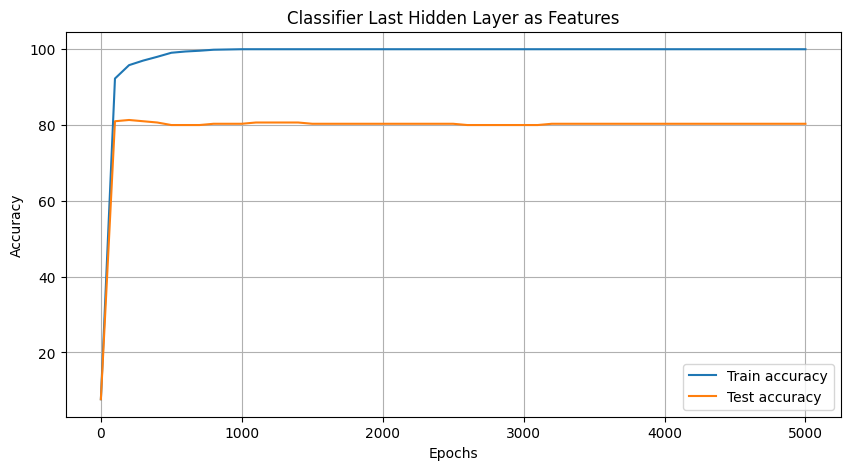
\includegraphics[width=.8\columnwidth]{images/1.2_last_hidden_layer.png}
    \caption{Test and train accuracy of the model}
    \label{fig-2}
\end{figure}

\pagestyle{OtherPage}
\subsection{Transfer learning -- Build a new network by replacing the last layer of PVMLNet with the weights of the
    trained perceptron.}
The last layer of PVMLNet was substituted with the weights obtained from the previously trained MLP network.
This approach, known as transfer learning, involves leveraging the knowledge acquired from training one model and applying it to another.\\
By replacing the last layer of PVMLNet with the weights of the MLP network, the researchers aimed to incorporate the learned representations
from the MLP into the deeper architecture of PVMLNet.
This strategy allows them to benefit from the specific features and patterns captured by the MLP, potentially improving the overall performance of PVMLNet.\\
Transfer learning is widely recognized as a powerful technique in machine learning as it enables the transfer of knowledge and generalization from one task to another.
By utilizing the pretrained MLP weights, the researchers aimed to enhance the predictive capabilities of PVMLNet,
leveraging the knowledge gained from the previous step to improve the classification accuracy for the cake image recognition task.
By doing so, the model reached a test accuracy of 80.67\%, which is a significant improvement over the previous models.

\section{Assignment}
\subsection{Combining features -- Try different combinations of low-level features (concatenate two or more feature vectors
    with np.concatenate).}
Combining multiple image processing techniques, such as the Histogram, Edge Direction Histogram, and passing them as features to the model,
can greatly enhance its performance. These techniques capture a richer set of information,
allowing the model to capture and utilize various patterns present in the images.\\
To explore the impact of different combinations of low-level features, various neural networks were trained using different feature sets.
These feature sets include the combination of Color Histogram and Edge Direction Histogram, RGB Co-occurrence Matrix and Co-occurrence Matrix,
and the combination of all four features.\\
The results in terms of test accuracy are depicted in Figure \ref{fig-3}.
It can be observed that the model utilizing all four low-level features performs significantly better compared to the other three models,
which exhibit similar performance levels.\\
This indicates that incorporating a comprehensive set of features can improve the model's ability to capture diverse image characteristics and patterns,
resulting in enhanced classification accuracy.
\begin{figure}[h]
    \centering
    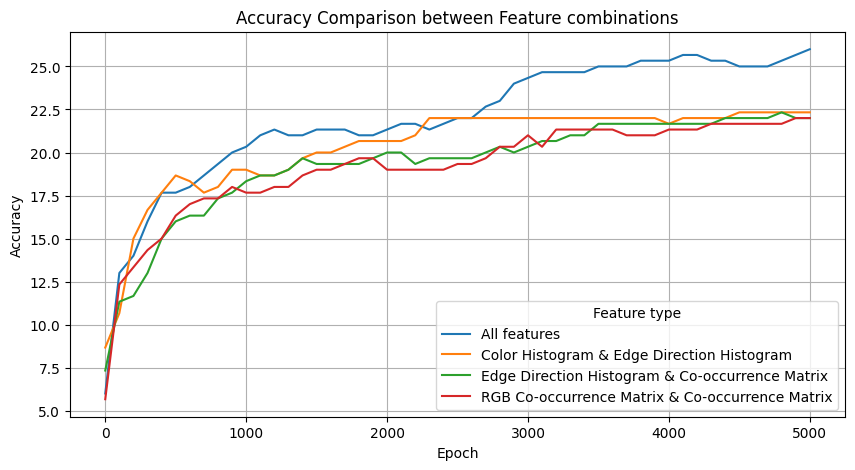
\includegraphics[width=.8\columnwidth]{images/2.1_diff_features.png}
    \caption{Test for the models trained with different features}
    \label{fig-3}
\end{figure}

\subsection{Analysis -- Identify the pairs of classes that are more likely to be confused with neural features.
    Also identify the test images that are misclassified even if the classifier predicted their
    label with high confidence.}
To thoroughly evaluate the performance of the model, it is essential to analyze the accuracy for each individual class rather than
solely relying on overall test and train accuracy.
The confusion matrix is a valuable tool for this analysis, as it displays the percentage of misclassifications from one class (y-axis) to another class (x-axis).\\
By examining the confusion matrix (see Figure \ref{fig-4}) for the model obtained by replacing the last layer of PVMLNet
with the weights of the trained perceptron, we can identify the classes that are most frequently misclassified.
Notably, the class 'chocolate mousse' exhibits the highest difficulty in recognition, often being confused with 'ice cream'.
Similarly, the class 'carrot cake' is frequently mistaken for 'tiramisu'.\\
To understand the reasons behind these misclassifications, a closer examination of images belonging to these classes is necessary
(see Figure \ref{fig-5}). It becomes apparent that 'carrot cake' and 'tiramisu' share similar color schemes, often comprising shades of brown and white.
Meanwhile, 'chocolate mousse' and 'ice cream' not only share similar colors but also have comparable shapes, contributing to the confusion between these two classes.\\
Furthermore, Figure \ref{fig-6} showcases the prediction errors made by the model, accompanied by the confidence levels associated with each prediction.
This visualization provides insights into the cases where the model's misclassifications occur, despite exhibiting high confidence.

\begin{figure}[h]
    \centering
    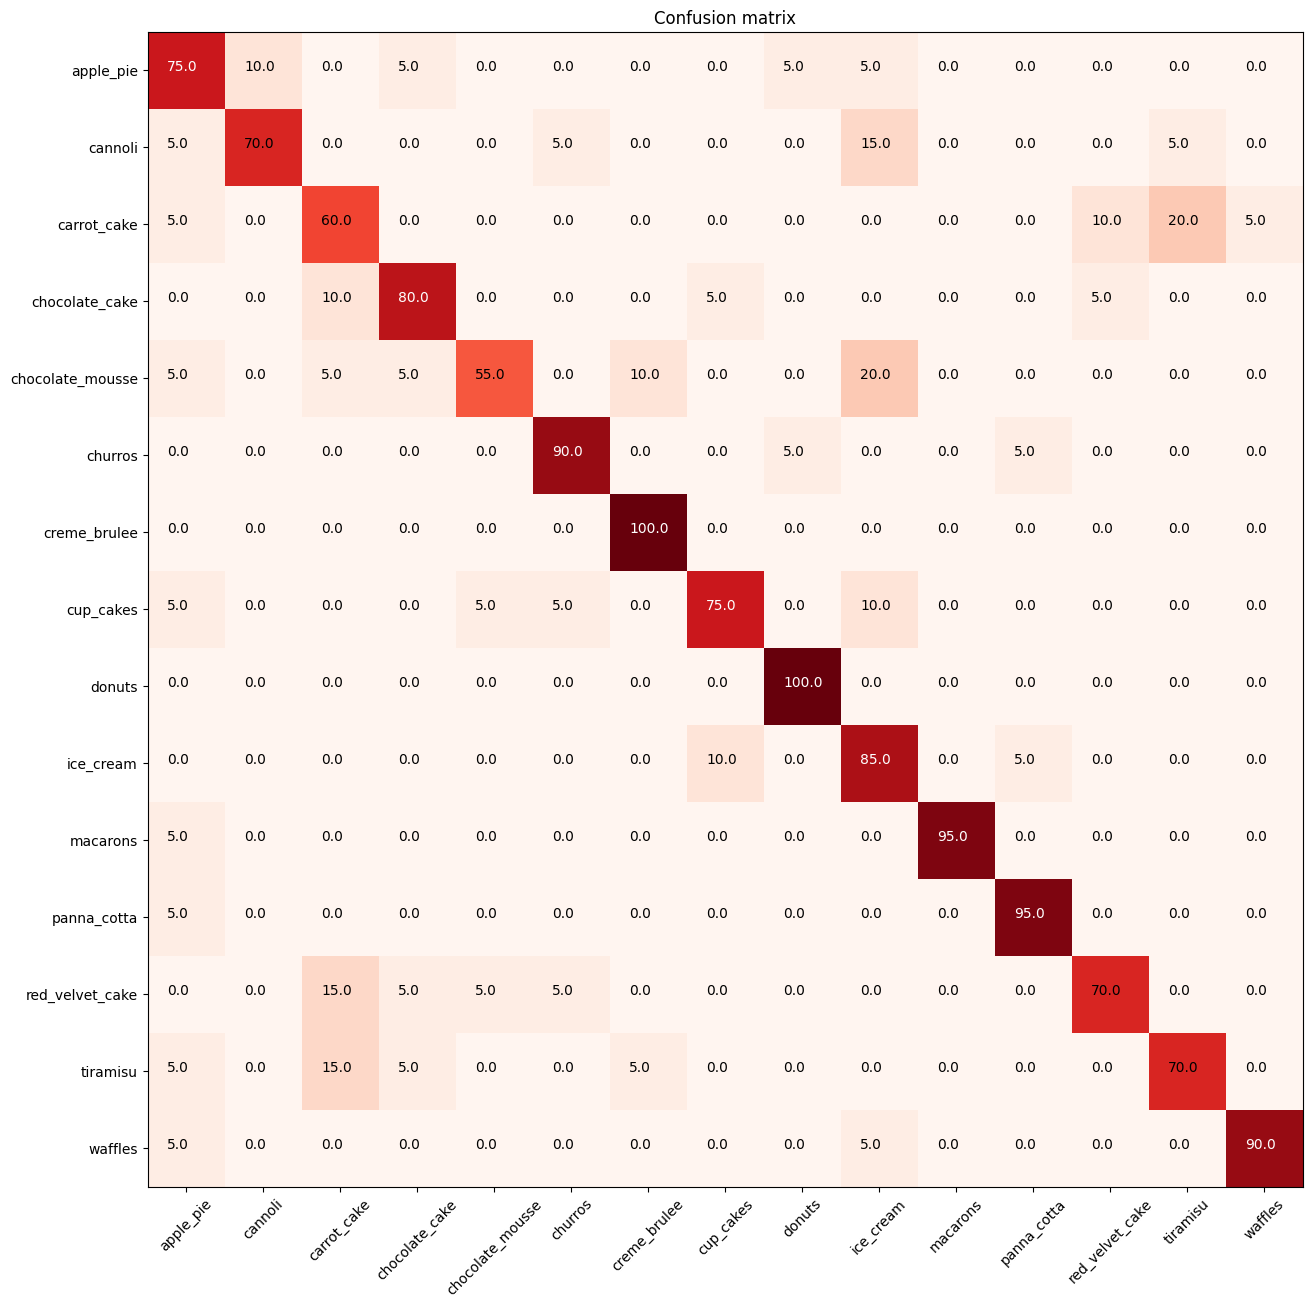
\includegraphics[width=\columnwidth]{images/2.2_confusion_matrix.png}
    \caption{Confusion matrix}
    \label{fig-4}
\end{figure}

\begin{figure}[h]
    \centering
    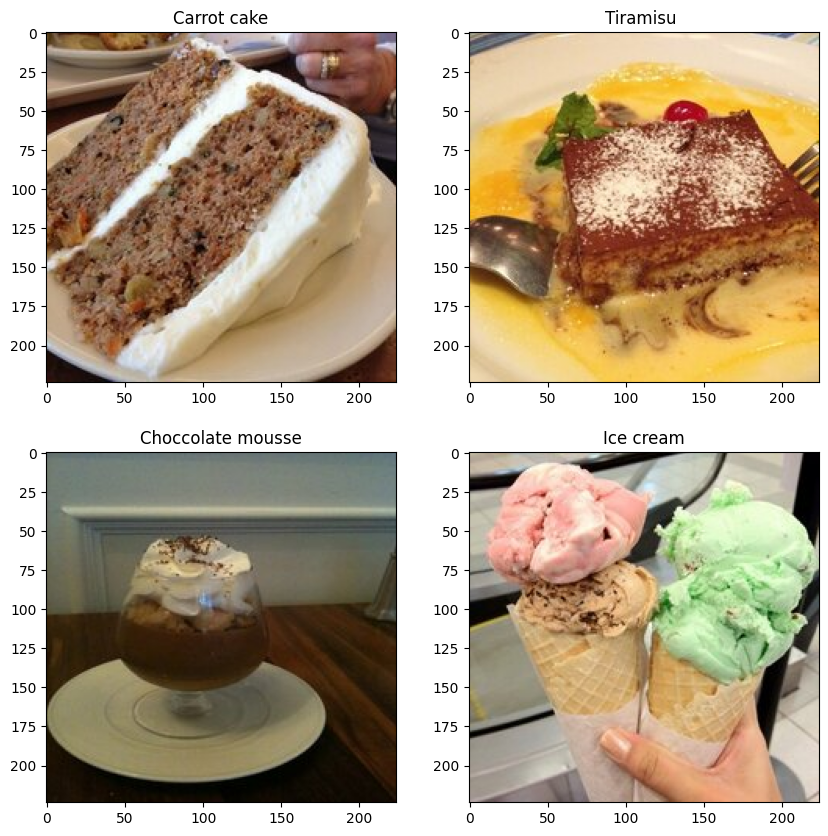
\includegraphics[width=.9\columnwidth]{images/2.2_sample_missclassified_cakes.png}
    \caption{Sample of the most misclassified cakes}
    \label{fig-5}
\end{figure}

\begin{figure}[h!]
    \centering
    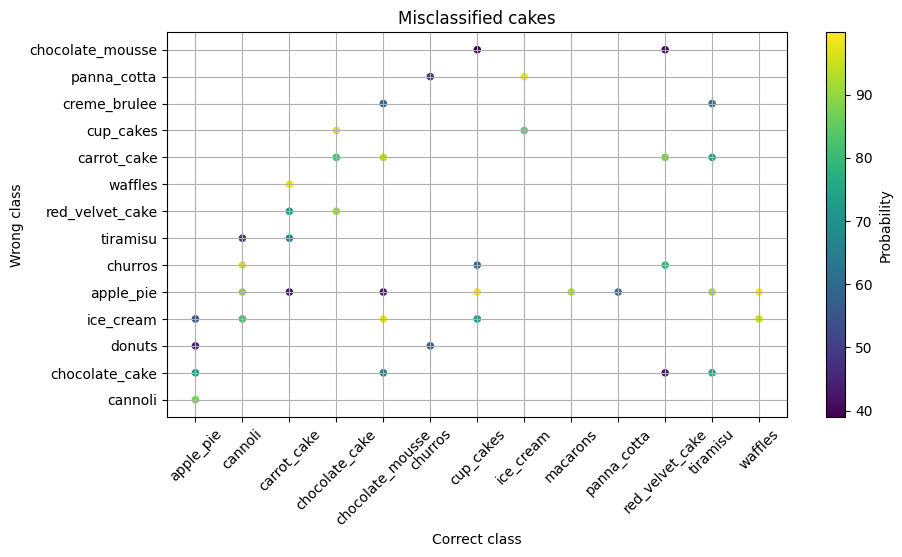
\includegraphics[width=.9\columnwidth]{images/2.2_probability_of_misclassified.png}
    \caption{Probability of misclassified cakes}
    \label{fig-6}
\end{figure}

\subsection{Neural features -- Try to use neural features computed by different hidden layers. When the activations
    are spatially distributed, you may reduce them to a single feature vector by averaging
    over the spatial dimensions.}
To analyze the information content and significance of the hidden layer activations, they were employed as features for an MLP neural network.
The influence of different layers on the accuracy of the final model is demonstrated in Figure \ref{fig-7}.\\
The choice of layer has a substantial impact on the performance of the model.
Notably, the fourth-to-last layer exhibits the highest accuracy of 85\%, followed by the third-to-last layer, the second-to-last layer,
and finally, the last layer, which demonstrates significantly lower performance.\\
\begin{figure}[h]
    \centering
    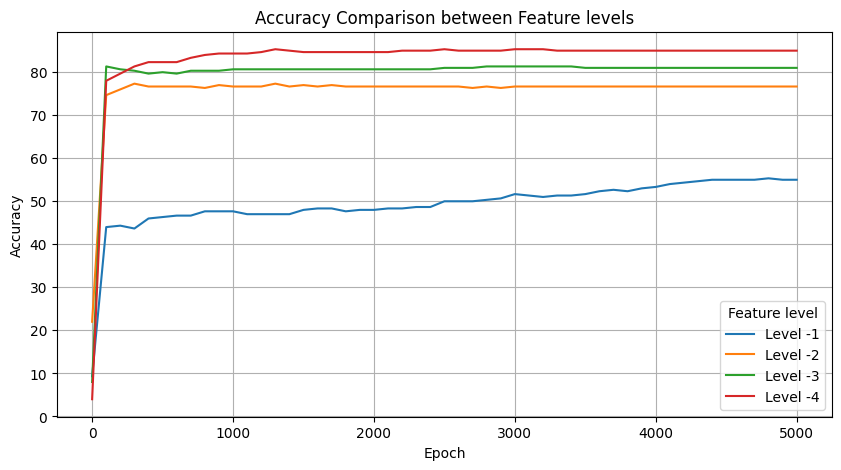
\includegraphics[width=.9\columnwidth]{images/2.3_diff_levels.png}
    \caption{Test accuracy for different hidden layers}
    \label{fig-7}
\end{figure}

\section{Declaration}
I affirm that this report is the result of my own work and that I did not share any part of it with anyone
else except the teacher.
\end{document}